\label{sec:app_concept}
%TODO Section{Idee/Gedankengänge/Planung} in der \subsectino{Konzept} mit den Wünschen des Users und die Benötigten Ressourcen und eine subsection{Komponenten} mit Unseren Komponenten/Ressourcen und wie sie miteinander funktionieren.

\subsection{Konzept}
Aus Perspektive der Benutzer ist die Idee hinter StreamSwipe trivial. Dem User werden nacheinander Filme und Serien vorgeschlagen, die er bewerten kann. Auf Basis seiner Präferenzen erhält er Matches, mit denen er über sich eine Chatfunktionen austauschen kann. Jeder dieser Schritte muss möglichst schnell und unkompliziert erfolgen.\\
Aus Sicht des Anbieters ist die Realisierung wesentlich komplexer als es dem User erscheint, da eine Zusammenstellung an Komponenten benötigt wird.  Diese besteht aus einer Smartphone-App, einer Userdatenbank, einer Datenbank mit den Filminformationen und einem Server, der das Matching ausführt. Zusätzlich wird eine mögliche Komponente für den Messenger benötigt. Die Auswahl dieser Komponente wird jeweils über individuell gestellte Anforderungen getroffen. \\

\noindent
Bei der Smartphone-App muss bereits während der Entwicklung auf Benutzerfreundlichkeit und Barrierefreiheit geachtet werden. Sie sollte intuitiv bedienbar, attraktiv designt und ressourcensparend für leistungsschwache Smartphones programmiert sein. Um ein möglichst großes Publikum ansprechen zu können, muss sie für iOS und Android erhältlich sein.\\
Die Datenbank mit den Benutzerinformationen muss jederzeit erreichbar sein und eine gewisse Form von Sicherheit und Verschlüsselung bieten, da da hier persönliche Angaben gespeichert werden.\\
Die Datenbank mit den Filminformationen  muss sehr umfangreich sein, also auch ältere Filme und Nischenfilme enthalten, und ständig aktualisiert werden. Neben den offensichtlichen Informationen wie Filmtitel und Filmposter muss sie auch weitere Daten zu den Filmen enthalten wie Erscheinungsdatum, Handlung, Regie, etc. trotzdem sollte der Zugriff schnell sein und nichts kosten, sodass die Nutzung der App möglichst preiswert ist.\\
Der Server muss durchgehend laufen und über eine Internetverbindung erreichbar sein. Er muss leistungsstark genug sein um alle Nutzeranfragen bedienen zu können, sollte jedoch so klein gehalten werden, dass die Anschaffungs- und Unterhaltskosten minimal sind.\\
Der Messenger  muss ebenfalls über einen zentralen Punkt gesteuert werden, da sich nur zwischen Personen ein Chat öffnen darf, die gematcht wurden. Es sollte keine Zugriffsbegrenzung auf diesen Server  geben, um einen unbegrenzten  Nachrichtenwechsel garantieren zu können. Nachrichten müssen gespeichert werden, um versendete Nachrichten auch nach dem Schließen der App zustellen zu können. Das System muss ebenfalls verschlüsselt sein und benötigt Zugriff auf Benutzerinformationen wie ID, Name und Profilbild.



X Server muss ständig laufen/erreichbar sein und Internetverbindung haben. In diesem Fall ein Raspberry Pi mit ... was eigentlich??? \\ %TODO Kapitel lesen!!!



\subsection{Komponenten}
\label{sec:komponenten}
In StreamSwipe ist für jede dieser Komponenten eine Lösung gefunden worden.
Bei der Entwicklung der App wurden Benutzerfreundlichkeit und Barrierefreiheit beachtet, wie in Abschnitt \ref{sec:UI-allgemein}, bzw. Abschnitt \ref{sec:barrierefreiheit} gezeigt wird. Wie in Abschnitt \ref{sec:framework} beschrieben wird, können die genannten Anforderungen durch eine geschickte Wahl des Frameworks erfüllt werden. Als Benutzerdatenbank kann Firebase verwendet werden, da wie in Abschnitt \ref{sec:firebase} beschrieben, die benötigten Funktionen vorhanden sind. Es ist ebenfalls möglich den Messenger mit den Firebasefunktionen zu implementieren. Als Quelle der Filminformationen wird die API von \glqq The Movie Database\grqq \, (TMDb) verwendet, auf welche in Abschnitt \ref{sec:filmdatenbank} genauer eingegangen wird. Der verwendete Server besteht aus einem Raspberry Pi, jedoch mehr dazu in Kapitel \ref{sec:server}. Wie diese Komponenten aufeinander zugreifen wird in Abbildung \ref{fig:komponentendiagramm} verdeutlicht.\\
Über die Smartphone-App werden die Benutzerdaten an Firebase weitergeleitet. Wird ein neuer Account angelegt, so werden diese Daten dort gespeichert und bei einem Anmeldevorgang sie mit den bestehenden Benutzerdaten verglichen. Nur wenn der User bereits vorhanden ist, kann eine Anmeldung stattfinden. So wird sichergestellt, dass nur angemeldete Benutzer auf die eigentlichen Funktionen der App Zugriff erhalten. Jede Aktion in der App wird auf diese Weise einem Benutzerkonto zugewiesen und kann später darüber identifiziert werden. Innerhalb der App können alle Funktionen frei genutzt werden weshalb es wichtig ist, dass ausschließlich eingeloggte User auf die Screens der App zugreifen können.\\
Der Server erhält die Film-IDs aller Filme aus der TMDb-API  und erstellt somit eine eigene Film-Datenbank. Diese IDs werden an das Smartphone weitergeleitet und die App erhält über die IDs die Filminformationen direkt von der TMDb-API. Es werden gleichzeitig nur eine geringe Anzahl an Filminformationen aus der TMDb-API auf das Smartphone geladen, sodass dieser Vorgang möglichst wenig Ressourcen benötigt und unbemerkt im Hintergrund ablaufen kann. Hierzu zählen Filmposter, Rating, Besetzung, Veröffentlichungsdatum, übersetzte Sprachen und viele mehr, die teilweise nicht benötigt werden. Noch bevor der User über alle diese Filme abgestimmt hat, werden neue Filminformationen geladen, sodass es für den User keine Unterbrechungen gibt und es ihm wie ein einzelner unendlicher Fluss an Daten erscheint. \\
Die Filmbewertung wird mit den Film-IDs vom Smartphone an den Server geschickt, der diese beiden Informationen miteinander verknüpft. Das Rekommendationsverfahren auf dem Server verarbeitet diese Präferenzen und sucht wie in Kapitel \ref{sec:recomandationSystem} beschrieben nach Übereinstimmungen bei den anderen Benutzern. Da hierbei alle Präferenzen aller User miteinander verglichen werden, ist dieser Schritt sehr aufwändig und sollte nicht nach jeder neuen Präferenz durchgeführt werden. Bei StreamSwipe wird dieses Matching deshalb automatisch in regelmäßigen Zeitabständen durchgeführt, optimalerweise zu einer Tageszeit, an der die Benutzeraktivität gering ist. Die Anzahl der verglichenen Nutzer kann mit einer Filterung durch Geschlechterpräferenzen und Wohnort reduziert werden um das Matchingverfahren zu beschleunigen. \\
Werden zwei User gematcht, wird dies ihnen jeweils in der App angezeigt. Die beiden Benutzer können dann einzeln entscheiden, ob sie die Unterhaltung starten wollen. Ist dies der Fall, werden die Nachrichten in der Firebase-Datenbank gespeichert. %TODO hier die abläufe des chats abklären!!!



%TODO Auch Leon fragen wie exakt das ganze abläuft
- Der Messenger kann ebenfalls über Firebase realisiert werden\\ %TODO Inwieweit gibts hier ein Kapitel drüber?

- Nutzer ID von beiden Nutzern bekannt bei der  Erstllung eines Chats
- Aus diesen beiden wird eine unique ID für den jeweiligen Chat erstellt und diese wird bei beiden Usern gespeichert
- (Firebase ist hierarchisch aufgebaut) Nutzernamen, NutzerID und RoomID werden in einer Sammlung gespeichert. Unter dieser Sammlung werden dann die Nachrichten abgespeichert mit den Informationen Wers gesendet hat, wers empfängt, einen tmestamp und natürlcih den inhalt der nachricht. sendby und sendto werden verwendet um die nachrichten im Chatverlauf anzuordnen und zu entscheiden welcher der beiden beteiligten eine benachrichtigung bekommt
- Anzeige der Chats abhängig davon ob die uniqueID in chatrooms oder pendingchatrooms gespeichert ist
- Wer die unterhaltung beginnt, erhält die unique ID in chatrooms und der andere in pendingchatrooms
- NImmt der andere User den Chat an, wird die ID für ihn ebenfalls in chtarooms verschioben
-


\begin{figure}[h]
\centering
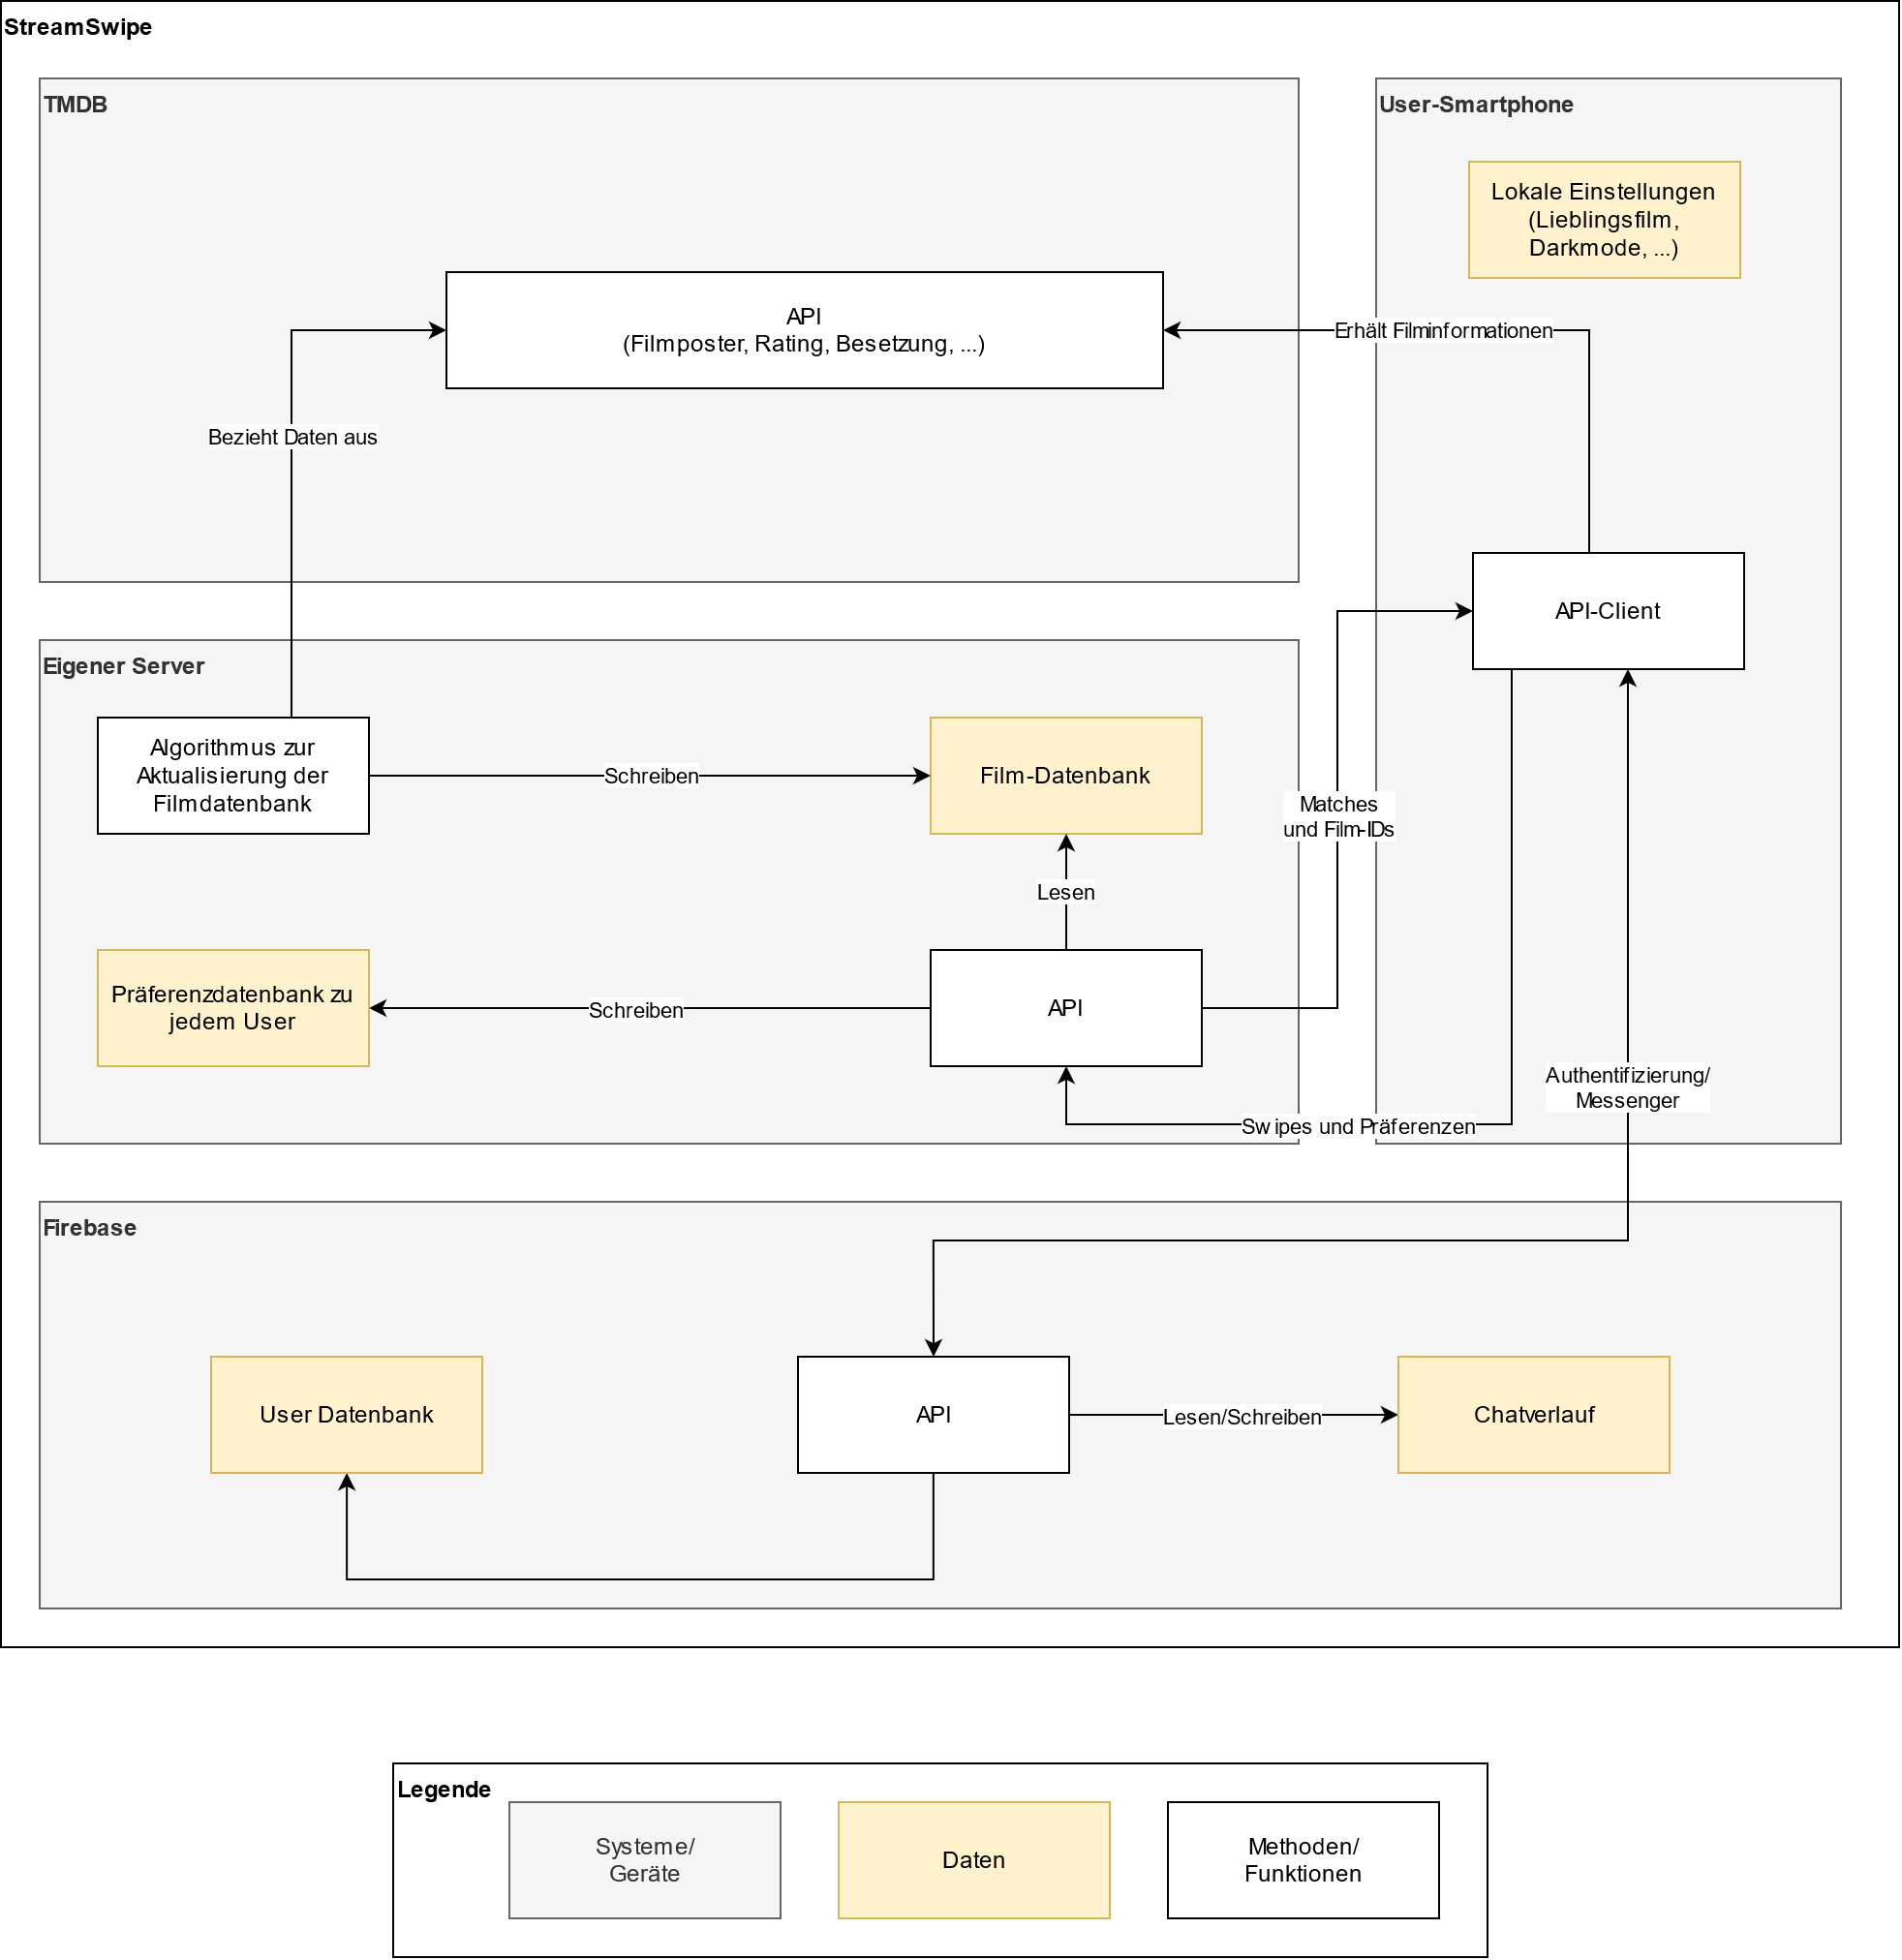
\includegraphics[width=16cm]{images/Konzeptdiagramm.png}
\caption{Komponentendiagramm}
\label{fig:komponentendiagramm}
\end{figure}